\chapter{Grundlagen}\label{chap:Grundlagen}

\section{Power-On-Reset-Schaltung}
Bei \glspl{ic} ist es wichtig, dass eine vordefinierte Anfangsbedingung bei Einschalten hergestellt wird. Besonders, wenn in dieser Schaltung Latches oder Speicherkomponenten integriert sind, muss eine  bekannte Anfangsbedingung sichergestellt werden, da sonst fehlerhafte Betriebszustände auftreten können. Sind die Betriebszustände nicht richtig initialisiert worden, kann es zu schwerwiegenden Timing-Problemen und zu Fehlverhalten innerhalb des \glspl{ic} führen. Damit diese Fehlzustände nicht auftreten, wird eine speziell für diesen Zweck konzipierte \gls{por}-Schaltung eingesetzt. Bei dieser wird ein internes Reset-Signal erzeugt, welches Komponenten wie Flip-Flops, Latches, Zähler und Register auf auf vordefinierte Werte zurücksetzt. So wird verhindert, dass sich das System in einem unbekannten Zustand befindet. Sobald der \gls{ic} an eine Versorgungsspannung angeschlossen wird, erkennt die \gls{por}-Schaltung den Spannungsanstieg und hält das Reset-Signal für eine gewisse Zeit ($t_{res}$) aktiv (siehe \autoref{fig:Schwellspannung}),
%\vspace{1.5\baselineskip}
\begin{figure}[H]
    \begin{center}
    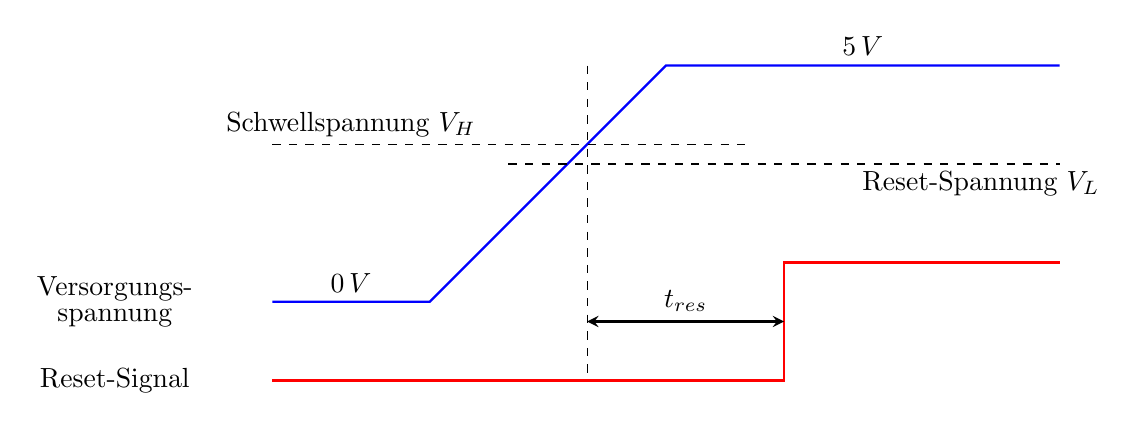
\begin{tikzpicture}
        % Achsen
        % \draw[->] (0,0) -- (10,0) node[anchor=north] {s}; % x-Achse
        % \draw[->] (0,0) -- (0,4) node[anchor=east] {V}; % y-Achse

        % Linie
        \draw[thick, blue] 
            (0,0) -- (2,0) % waagerechter Teil von 0 bis 2 Sekunden
            to (5,3) -- ++(5,0);
            % Kreuzungspunkt berechnen
        \coordinate (Kreuzung) at (4,2);

        
        \draw[thick, red] 
            (0,-1) -- ++(6.5,0) -- ++(0,1.5) -- ++(3.5,0);

        % Gestrichelte Linien
        \draw[dashed] 
            (0,2) -- ++ (6,0); % Senkrechte Linie nach unten
        \draw[dashed] 
            (4,3) -- ++(0,-4); % Waagerechte Linie nach rechts
        \draw[dashed] 
            (3,1.75) -- ++(7,0);
            
        % Beschriftungen
        \node[anchor=south, xshift=1cm] at (0,0) {$0\,V$}; % Startpunktbeschriftung
        \node[anchor=south] at (7.5,3) {$5\,V$}; % Endpunktbeschriftung
        \node[] at (-2,0) {\shortstack{Versorgungs- \\spannung}};
        \node[] at (-2,-1) {\shortstack{Reset-Signal}};
        \node[] at (1,2.25) {\shortstack{Schwellspannung $V_H$}};
        \node[] at (9,1.5) {\shortstack{Reset-Spannung $V_L$}};


        \draw[<->, thick, >=stealth] (4,-0.25) -- ++(2.5,0) node[midway, above] {$t_{res}$}; % Pfeil

        
    \end{tikzpicture}        

    \end{center}
    \caption[Schwellspannung]{\\Quelle: Schwellspannung (Eigene Darstellung)}
    \label{fig:Schwellspannung}
\end{figure}
%\vspace{1.5\baselineskip}
damit sich alle auf dem \acrlong{ic} befindlichen Komponenten stabilisieren können. Diese Verzögerung ist außerdem notwendig, um eine zu frühe Freigabe des Reset-Signals zu verhindern, wenn zu Schwankungen oder Spannungsspitzen während der Initialisierungsphase kommt. Nachdem die Verzögerung ($t_{res}$) des Reset-Signals frei gibt, geht das System in den normalen Betriebsmodus über. Die Verzögerungszeit beginnt erst nachdem, eine gewisse Schwellspannung ($V_H$) erreicht ist, damit ein sicherer Betrieb des \glspl{ic} gewährleistet werden kann. Wenn es während des Betriebs zu einem unvorhersehbaren Spannungsabfall kommt,  kann auch das zu einem fehlerhaften Betriebszustand führen, weshalb ein erneuter Reset unverzichtbar ist  (siehe \autoref{fig:Reset-Spannung}). Entscheidend dafür ist, dass die Reset-Spannung ($V_L$) unter der Schwellspannung ($V_H$) für das Reset-Signal liegt. Sobald die Versorgungsspannung unter den Schwellenwert der Reset-Spannung fällt, soll die \gls{por}-Schaltung möglichst ohne Verzögerung den Reset auslösen \cite{9647518}. 
%\vspace{1.5\baselineskip}
\begin{figure}[H]
    \begin{center}
    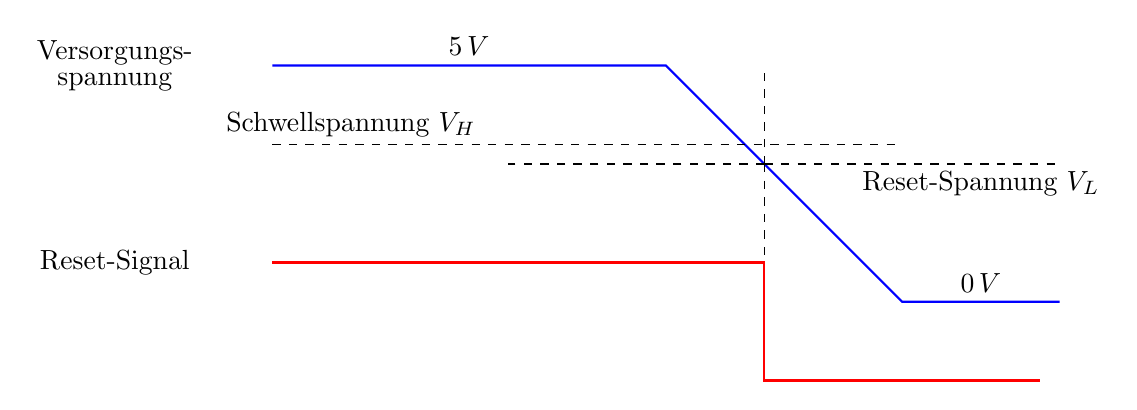
\begin{tikzpicture}
        % Achsen
        % \draw[->] (0,0) -- (10,0) node[anchor=north] {s}; % x-Achse
        % \draw[->] (0,0) -- (0,4) node[anchor=east] {V}; % y-Achse

        % Linie
        \draw[thick, blue] 
            (0,3) -- (5,3) % waagerechter Teil von 0 bis 2 Sekunden
            to (8,0) -- ++(2,0);
            % Kreuzungspunkt berechnen
        \coordinate (Kreuzung) at (6.25,1.75);

        
        \draw[thick, red] 
            (0,0.5) -- ++(6.25,0) -- ++(0,-1.5) -- ++(3.5,0);

        % Gestrichelte Linien
        \draw[dashed] 
            (Kreuzung) -- ++ (-3.25,0)
            (Kreuzung) -- ++ (3.75,0); % Waagerechte Linien
        \draw[dashed] 
            (Kreuzung) -- ++(0,-1.25)
            (Kreuzung) -- ++(0,1.25); % Senkrechte Linien
        \draw[dashed] (0,2) -- ++ (8,0); % Schwellspannung
            
        % Beschriftungen
        \node[anchor=south, xshift=-1cm] at (10,0) {$0\,V$}; % Startpunktbeschriftung
        \node[anchor=south] at (2.5,3) {$5\,V$}; % Endpunktbeschriftung
        \node[] at (-2,3) {\shortstack{Versorgungs- \\spannung}};
        \node[] at (-2,0.5) {\shortstack{Reset-Signal}};
        \node[] at (1,2.25) {\shortstack{Schwellspannung $V_H$}};
        \node[] at (9,1.5) {\shortstack{Reset-Spannung $V_L$}};
        
    \end{tikzpicture}        

    \end{center}
    \caption[Reset-Spannung]{\\Quelle: Reset-Spannung (Eigene Darstellung)}
    \label{fig:Reset-Spannung}
\end{figure}
%\vspace{1.5\baselineskip}

\section{Differenzverstärker und Komparator}
Ein Komparator (siehe \autoref{fig:Komp}) wird eingesetzt, um zwei analoge Eingangssignale \mbox{($V_{inn}$ und $V_{inp}$)} zu vergleichen und abhängig vom Vergleich einen entsprechendes binäres Ausgangssignal ($V_{out}$) zu liefern. Der Komparatorausgang kann dabei unregelmäßig werden, wenn die Eingangssignale zu stark rauschen. Dieses Rauschen ist ein unerwünschtes Signal, welches nicht mit den Eingangssignal zusammenhängt \cite{7489413}. 
%\vspace{1.5\baselineskip}
\begin{figure}[H]
    \begin{center}
        \begin{circuitikz}[european]
            \ctikzset{tripoles/mos style/arrows}[line width=thick, european]
            % Komparator    
            \draw (0,0) node[op amp] (triangle){}; 
            \draw (triangle) node[above, yshift=27pt] {Komparator};
            \draw (triangle.out) -- ++(1,0) node[above]{$V_{out}$};    
            \draw (triangle.+) -- ++(-1,0) node[above]{$V_{inp}$};
            \draw (triangle.-) -- ++(-1,0) node[above]{$V_{inn}$};

            \draw (7,0.5) node[]{$V_{inp} > V_{inn}$ \hspace{5pt} \textbf{dann} \hspace{5pt} $V_{out} = V_{DD} =$ logische 1};
            \draw (7,-0.5) node[]{$V_{inp} < V_{inn}$ \hspace{5pt} \textbf{dann} \hspace{5pt} $V_{out} = 0 =$ logische 0};

        \end{circuitikz}
    \end{center}
    \caption[Schaltzeichen Komparator]{\\Quelle: Eigene Darstellung Schaltzeichen Komparator in Anlehnung an \cite[S. 909]{CircuitDesigLayoutAndSimulation}}
    \label{fig:Komp}
\end{figure}
% \vspace{1.5\baselineskip}
In einer \gls{por}-Schaltung kann man sich den Komparator als Entscheidungsschaltung vorstellen. Sobald die Betriebsspannung ($V_{inp}$) ein größeres Potential als die Referenzspannung ($V_{inn}$) hat, erhält man am Ausgang des Komparators ($V_{out}$) eine logische 1. Wenn die Betriebsspannung ein niedrigeres Potential aufweist als die Referenzspannung, dann erhält man eine logische 0 am Komparatorausgang \cite{CircuitDesigLayoutAndSimulation}.

\section{Schmitt-Trigger}
Bei nicht Schmitt-getriggerten Bauteilen findet der Schaltvorgang der steigenden und fallenden Flanke immer am gleichen Punkt statt. Bei einem rauschenden Eingangssignal kann der Schwellenwert mehrfach überschritten werden, wodurch eine Mehrfachtaktung oder Oszillation auftreten kann. Dadurch kann es zu einem übermäßigen Stromfluss im gesamten Bauteil kommen. Damit diese Probleme nicht auftreten wird ein Schmitt-Trigger (siehe \autoref{fig:ST_symbol}) verwendet. 
%\vspace{1.5\baselineskip}
\begin{figure}[H]
    \begin{center}
        \begin{circuitikz}[european]
            \ctikzset{tripoles/mos style/arrows}[line width=thick, european]
             % Schmitt-Trigger mit Eingangs- und Ausgangsbezeichnung
            \draw (-4,1) node[schmitt] (schmitt){}; 
            \draw (schmitt) node[above, yshift=27pt] {Schmitt-Trigger};
            
            \draw (schmitt.in) -- ++(-1,0) node[above]{$V_{in}$}; % Eingangsleitung
            \draw (schmitt.out) -- ++(1,0) node[above]{$V_{out}$}; % Ausgangsleitung

            \draw[->, thick] (0,0) -- ++(0,4) node[above]{$V_{out}$}
                coordinate[pos=5/6](VDDy);
                \draw (VDDy) node[left]{\tiny{$V_{DD}$}};
            
            \draw[->, thick] (0,0) -- ++(4,0) node[right]{$V_{in}$}
                coordinate[pos=2/7](VL)
                coordinate[pos=5/7](VH)
                coordinate[pos=10/11](VDD);

            \draw (VDD) -- ++(0,0.1)
                (VDD) -- ++(0,-0.1) node[below]{\tiny{$V_{DD}$}};

            \draw[rounded corners=5pt] (VDDy) -| (VL) -- (VDD);
            \draw[->] (VL) ++(0,2.5) -- ++(0,-2pt);
            \draw[->] (VL) ++(0,0.75) -- ++(0,-2pt);

            \draw[rounded corners=5pt] (VDDy) -| (VH) -- (VDD);
            \draw[->] (VH) ++(0,2.5);
            \draw[->] (VH) ++(0,0.75);
            
            \draw (VH) node[below, xshift=5pt]{\tiny{$V_H$}};
            \draw (VL) node[below, xshift=5pt]{\tiny{$V_L$}};

        \end{circuitikz}
    \end{center}
    \caption[Symbol Schmitt-Trigger]{\\Quelle: Eigene Darstellung Symbol Schmitt-Trigger in Anlehnung an \cite[S. 909]{CircuitDesigLayoutAndSimulation}}
    \label{fig:ST_symbol}
\end{figure}
%\vspace{1.5\baselineskip}
Hauptmerkmal dieses Bauteils ist die Hysterese, welche als Rauschunterdrückung fungiert. Die Schwellenwerte sind so eingestellt, dass die steigende Flanke an einem höheren Punkt ($V_H$) und die fallende Flanke an einem niedrigeren Punkt ($V_L$) schaltet. Die Differenz der beiden Schaltpunkte wird als Hysterese bezeichnet und lässt sich durch das Verhältnis der Transistoren eingestellt werden \cite{CMOS_VLSI_Design}\cite{CircuitDesigLayoutAndSimulation}\cite{texasST}.

\section{Transistoren}
Ein \gls{cmos} ist einer der Schlüsselkomponenten auf heutigen \glspl{ic}. Diese basieren auf der Technologie von \gls{mosfet} und werden als komplementär bezeichnet, da die Kanäle der Transistoren ein komplementäres Paar bilden. \glspl{mosfet} leiten unter bestimmten Bedinungen Strom, da sie aus Halbleitermaterialien bestehen. In der Regel bestehen sie aus Silizium, welches in seiner reinen Form nicht leitfähig ist, und einer Mischung aus Verunreinigungen, wodurch eine Leitfähigkeit erzeugt wird. Abhängig von den Verunreinigungen kann man \gls{mosfet}-Halbleiter in p-Typ und n-Typ unterscheiden. Üblicherweise wird Bor, Gallium und Indium für den p-Typ verwendet und Phosphor, Arsen und Wismut für den n-Typ. Die Halbleiter mit der p-typischen Verunreinigung sind positiv geladen, im Gegensatz dazu besitzen die n-Typen eine negative Ladung. Daraus ergeben sich auch die beiden Haupttypen von \gls{mosfet}-Transistoren \cite{What_is_CMOS}\cite{Göbel2019}. 

In \autoref{fig:nmos_structure} wird der allgemeine Aufbau eines \gls{mosfet}-Transistors mit n-Kanal dargestellt, welcher als \gls{nmos} bezeichnet wird. Das Halbleitergrundmaterial, welches als Substrat bzw. Bulk ($B$) bezeichnet wird, ist p-dotiert und somit gegensätzlich zu der n-Dotierung von Source ($S$) und Drain ($D$). 
\input{figures/Schaltkreise/nmos_structure}
Wenn eine positive Spannung $U_{DS}$ zwischen Source und Drain angelegt wird, sind die beiden pn-Übergänge in Sperrrichtung. Damit ein Strom ($I_{DS}$) zwischen Drain und Source fließen kann, muss eine positive Spannung an das Gate ($G$) angelegt werden. In diesem Fall, lädt sich die Elektrode am Gate positiv auf. Dadurch bildet sich unterhalb der Oxidschicht eine aus Elektronen bestehende Gegenladung. Aufgrund dessen verhält sich der p-Halbleiter wie ein n-dotierter Halbleiter. Die Grenzschicht, die zwischen dem Oxid und dem Halbleiter entsteht, bildet einen Kanal. Dieser verbindet Source und Drain, wodurch der Stromfluss $I_{DS}$ ermöglicht wird \cite{Göbel2019}. 

Die \autoref{fig:MOSFET_Transferkennlinie} zeigt das Symbol eines \gls{nmos}-Transistors und die dazugehörige Transferkennlinie. Diese Kennlinie zeigt den Drainstrom $I_D$ in Abhängigkeit von der Gate-Source-Spannung $V_{GS}$ bei konstantem $V_{DS}$. Wenn $V_{GS}$ eine bestimmte Schwelle $V_{th}$ überschreitet, bildet sich ein leitender Kanal, und Strom kann zwischen Drain und Source fließen.
\begin{figure}
    \centering
    \begin{tikzpicture}
    \ctikzset{tripoles/mos style/arrows}[line width=thick, european]
´         % NMOS-Transistor-Symbol auf der linken Seite
        \begin{scope}[xshift=-3cm] % Verschiebung des Symbols nach links
            \draw (0,2) node[nmos](nmos){};
            \node[above] at (nmos.gate) {$G$}
                (nmos.gate) -- ++(-0.1,0) coordinate(gate)
                node[circle, draw,inner sep=1.5pt]{};
            \node[below, yshift=-5pt] at (nmos.source) {$S$}
                (nmos.source) -- ++(0,-0.1) coordinate(source)
                node[circle, draw,inner sep=1.5pt]{};
            \node[left] at (nmos.drain) {$D$}
                (nmos.drain) -- ++(0,0.1) coordinate(drain)
                node[circle, draw,inner sep=1.5pt]{};

            \draw[->, shorten >=5pt, shorten <=5pt, >=stealth] (drain) to[out=-45,in=45] (source)
                node[xshift=22pt, yshift=25pt]{\footnotesize{$V_{DS}$}};
            \draw[<-, shorten <=5pt, >=stealth] (drain) -- ++ (0,.75) 
                node[right, midway, yshift=5pt]{\footnotesize{$I_D$}};
            \draw[->, shorten >=5pt, shorten <=5pt, >=stealth] (gate) to[out=-90,in=180] (source)
                node[xshift=-25pt]{\footnotesize{$V_{GS}$}};
            \fill[white] (2,1) rectangle (2.975,0);
        \end{scope}

        \begin{axis}[
            xlabel={$V_{GS}$},
            ylabel={$I_D$},
            xmin=0, xmax=4,
            ymin=0, ymax=300,
            xtick=\empty, % Entfernt die Ticks und Beschriftungen der X-Achse
            ytick=\empty,
            width=7cm,
            height=6cm,
            %title={MOSFET Transferkennlinie},
            %title style={yshift=10pt}, % Abstand zwischen Titel und Grafik erhöhen
            %legend pos=north west,
            axis lines=middle, % Achsen in der Mitte mit Pfeilen
            xlabel style={at={(ticklabel* cs:1)}, anchor=north west, xshift=-10pt}, % Beschriftung neben    dem Pfeil
            ylabel style={at={(ticklabel* cs:1)}, anchor=south east, yshift=-10pt}, % Beschriftung neben    dem Pfeil
            minor tick num=0, % Schrittweite entfernen
            minor y tick num=0,
            extra x ticks={1.5}, % Markierung bei V_GS = 1.5
            extra x tick labels={$V_{th}$}, % Beschriftung der Markierung
            extra x tick style={
                grid=none, % Keine Gitterlinie bei der Markierung
                tick pos=left % Tick auf der linken Seite der Achse
            }
        ]
        
        % Beispiel: Quadratische Kennlinie im Sättigungsbereich
        \addplot[
            domain=1.5:4, % V_GS von 1V bis 7V
            samples=100,
            color=blue,
            thick,
        ] {150 * (x - 1.5)^4}; 
        \addplot[
            domain=0:1.5,
            samples=100,
            color=blue,
            thick,
        ] {0};
    
    
        \addplot[
            domain=1.5:4, % V_GS von 1V bis 7V
            samples=100,
            color=red,
            thick,
            style=dashed
        ] {100 * (x - 1.5)^4};
    
        \addplot[
            domain=1.5:4, % V_GS von 1V bis 7V
            samples=100,
            color=red,
            thick,
            style=dashed
        ] {250 * (x - 1.5)^4};
        
        \end{axis}
    \end{tikzpicture}
    \caption[Symbol NMOS-Transistor mit Transferkennlinie]{\\Quelle: Eigene Darstellung Symbol NMOS-Transistor mit Transferkennlinie in Anlehnung an \cite[S. 268]{MicroelectronicCircuits}}
    \label{fig:MOSFET_Transferkennlinie}
\end{figure}
Für die Berechnung des Drainstroms im Sättigungsbereich (wenn $V_{DS} \geq V_{GS} - V_{TH}$) wird diese Formel verwendet: 
\begin{equation}
    I_D = \beta (V_{GS} - V_{TH})^2
\end{equation}
\begin{equation}
    \beta = \alpha \frac{W}{L}
\end{equation}
\begin{equation}
    \alpha = \frac{1}{2} \mu_n C_{ox}
\end{equation}
Die Prozessparameter $\mu_n$ und $C_{ox}$ geben die Beweglichkeit der Ladungsträger und die Oxidkapazität pro Flächeneinheit an und lassen sich während des Schaltungsentwurfs nicht beeinflussen. Durch gezielte Anpassung der Kanalbreite ($W$) und Kanallänge ($L$) können die elektrischen Eigenschaften der \gls{mosfet}-Transistoren beeinflusst werden. Eine größere Kanalbreite ($W$) führt zu einer gesteigerten Stromfähigkeit des Transistors, da auf einem breiteren Kanal mehr Ladungsträger transportiert werden können. Dies führt außerdem zu einem gesteigerten Drainstorm ($I_D$), wodurch die Schaltgeschwindigkeit verbessert wird. Allerdings steigt dadurch eine größere Kanalbreite auch der Energieverbrauch. Die Kanallänge ($L$) hingegen beeinflusst den Widerstand des Kanals. Eine kürzere Kanallänge reduziert diesen Widerstand und erhöht die Geschwindigkeit des Transistors. Dadurch können aber kurz Kanal-Effekte auftreten, die zu erhöhten Leckströmen und Instabilität führen können. Aus diesen Gründen muss ein Kompromiss zwischen Leistung, Energieverbrauch und Stabilität gefunden werden, weshalb eine gezielte Anpassung des $W/L$-Verhältnis notwendig ist \cite{MicroelectronicCircuits}.
    
Der Aufbau eines p-Kanal \gls{mosfet} ist grundsätzlich der gleiche wie beim \gls{nmos}, jedoch ist die Dotierung umgekehrt (siehe \autoref{fig:pmos_structure}). Das Substrat ist n-dotiert und die \mbox{Source-/Draingebiete} p-dotiert, was eine Umkehr der Vorzeichen zur Folge hat. 
%\vspace{1.5\baselineskip}
\begin{figure}[H]
    \begin{center}
        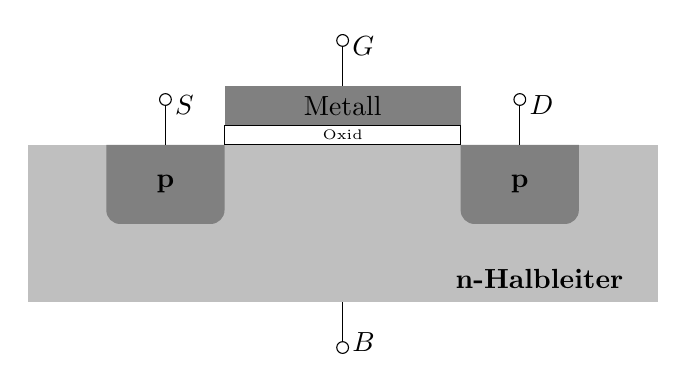
\begin{tikzpicture}
            % N-Type Substrate
            \fill[lightgray] (-4,1) rectangle (4,-1);
            \node at (2.5,-.7) {\textbf{n-Halbleiter}};
            
            % P+ regions
            \fill[gray]
                (-3,1) -- (-1.5,1) -- 
                ++(0,-0.83) arc[start angle=0, end angle=-90, radius=5pt] -- 
                ++(-1.15,0) arc[start angle=-90, end angle=-180, radius=5pt] -- 
                cycle;
            \node at (-2.25,0.5) {\textbf{p}};
            \fill[gray]
                (1.5,1) -- (3,1) -- 
                ++(0,-0.83) arc[start angle=0, end angle=-90, radius=5pt] -- 
                ++(-1.15,0) arc[start angle=-90, end angle=-180, radius=5pt] -- 
                cycle;
            \node at (2.25,0.5) {\textbf{p}};

            % Gate
            \fill[gray]
                (-1.5,1.75) rectangle (1.5,1.25);
            \node at (0,1.5) {{Metall}};
            \draw (-1.5,1.25) rectangle (1.5,1)
                node at (0,1.125) {\tiny{Oxid}};
            \draw (0,1.75) -- ++(0,0.5)   
                node[circle, draw,inner sep=1.5pt] at (0,2.325){}
                    node[right]{$G$};

            % Source 
            \draw (-2.25,1) -- ++(0,0.5)   
                node[circle, draw,inner sep=1.5pt] at (-2.25,1.575){}
                    node[right]{$S$};
                    
            % Drain 
            \draw (2.25,1) -- ++(0,0.5)   
                node[circle, draw,inner sep=1.5pt] at (2.25,1.575){}
                    node[right]{$D$};

            % Bulk
            \draw (0,-1) -- ++(0,-0.5)   
                node[circle, draw,inner sep=1.5pt] at (0,-1.575){}
                    node[right]{$B$};
                    
        \end{tikzpicture}
    \end{center}
    \caption[Struktur PMOS-Transistor]{\\Quelle: Eigene Darstellung Struktur PMOS-Transistor in Anlehnung an \cite[S. 107]{Göbel2019}}
    \label{fig:pmos_structure}
\end{figure}
% \vspace{1.5\baselineskip}
Wenn beispielsweise 0 V an Gate und Drain sowie 5~V an Source und Bulk, ergibt sich eine negative Gate-Source-Spannung $U_{GS}$ von -5 V. Da $U_{DS}$ auch eine negative Spannung hat, fließt ein negative Drain-Source Strom $I_{DS}$. Dabei ist zu beachten, dass sowohl für den \gls{nmos} als auch für den \gls{pmos} eine gewisse Schwellspannung überschritten werden muss, damit sich der Kanal zwischen Source und Drain bilden kann~\cite{Göbel2019}.  

Native Transistoren, zeichnen sich durch eine sehr geringe Schwellspannung nahe Null aus. Diese Eigenschaft unterscheidet sie grundlegend von herkömmlichen Transistoren, die eine bestimmte Gate-Source-Spannung benötigen, um Strom zu leiten. Damit dies möglich ist, wird die Dotierung im Kanalbereich angepasst. Bei einem \gls{nmos}-Transistor ist der Kanal leicht n-dotiert, anstatt p-dotiert. Aufgrund dessen ist ein Native Transistor bereits ohne angelegte Gate-Source-Spannung leitfähig, was ihn besonders für Anwendungen in einer Low-Power-Schaltung nützlich macht \cite{Evolution}.

\section{Stromspiegel}
Ein Stromspiegel (siehe \autoref{fig:current_mirror}) ist eine grundlegende Schaltung im analogen \gls{ic}-Entwurf, die dazu dient, einen definierten Strom ($I_{in}$) von einem Referenzzweig auf einen Ausgangszweig ($I_{out}$) zu übertragen.
%\vspace{1.5\baselineskip}
\begin{figure}[H]
    \begin{center}
        \begin{circuitikz}[european]
            \ctikzset{tripoles/mos style/arrows}[line width=thick, european]
            
            % Transistoren 
            \draw (-2,0) node[nmos, yscale=-1, rotate=180](nmosL){}
                node at (nmosL.center) [anchor=center, xshift=-10pt]{$N_0$};
            \draw (2,0) node[nmos](nmosR){$N_1$};

            \draw (nmosL.gate) -- (nmosR.gate)
                coordinate[pos=0.5](gate_cross)
                (gate_cross) node[circle, fill, inner sep=1.5pt]{};

            \draw (nmosL.drain) -- ++(0,0.25) 
                coordinate(left_cross)
                node[circle, fill, inner sep=1.5pt]{};

            \draw (left_cross) -| (gate_cross);

            \draw (left_cross) -- ++(0,1.25);
            \draw (nmosR.drain) -- ++(0,1.5);

            % Ground 
            \draw (nmosL.source) -- ++ (0,-0.5) -- ++ (2,0)
                node[circle, fill, inner sep=1.5pt]{};
            \draw (nmosR.source) -- ++ (0,-0.5) -- ++ (-2,0)
                coordinate(ground);
            \draw (ground) -- ++(0,-.25) node[sground]{}
                node[right, xshift=5pt, yshift=-7pt]{Gnd};

            % Ströme
            \draw[->, thick, >=stealth] (-2.25,2) -- ++(0,-.75)
                node[left, yshift=10pt]{$I_{in}$};
            \draw[->, thick, >=stealth] (2.25,2) -- ++(0,-.75)
                node[right, yshift=10pt]{$I_{out}$};

        \end{circuitikz}
    \end{center}
    \caption[Aufbau Stromspiegel]{\\Quelle: Eigene Darstellung Aufbau Stromspiegel in Anlehnung an \cite[S. 512]{MicroelectronicCircuits}}
    \label{fig:current_mirror}
\end{figure}
Dadurch ist der Stromspiegel eine wichtige Komponente im analogen Schaltungsentwurf, insbesondere für Referenzstromquellen und Differenzverstärker. Ein typischer Stromspiegel besteht aus zwei \gls{mosfet}-Transistoren, die so verbunden sind, dass einer als Referenztransistor ($N_0$) und der andere als Lasttransistor ($N1$) agieren. Da beide Transistoren die gleiche Gate-Source-Spannung ($V_{GS}$) besitzen, ist auch der Drainstrom ($I_D$) identisch. Haben die Transistoren $N_1$ und $N_2$ das gleiche $W/L$-Verhältnis, so wird der Strom $1:1$ gespiegelt ($I_{out} = I_{in}$). Der Ausgangsstrom ($I_{out}$) wird durch das $W/L$-Verhältnis der Transistoren beeinflusst und kann durch folgende Gleichung berechnet werden: 
\begin{equation}
    \frac{I_{in}}{I_{out}} = \frac{(W/L)_{N_0}}{(W/L)_{N_1}} \Rightarrow I_{out} = I_{in} \frac{(W/L)_{N_1}}{(W/L)_{N_0}}
\end{equation}dia